\subsection{Sistema \acrshort{GSM}}
\label{sub:GSM}
El sistema \acrshort{GSM} tiene está definido por las siguientes características:
\begin{itemize}
	\item Modulación GMSK
	\item Una protección cocanal $\frac{C}{I}=9dB$
	\item Una protección contra dispersión dopler capaz de mantenerse hasta a 200 km/h
	\item Una interferencia base con 6 celdas $i_0=6$
	\item Se trata de un sistema \acrshort{FDD}/\acrshort{FDMA}/\acrshort{TDMA}
	\begin{itemize}
		\item \acrshort{FDD} la subida y bajada se encuentran separadas en diferentes bandas de frecuencia
		\item \acrshort{FDMA}/\acrshort{TDMA} los canales se encuentran en diferentes frecuencias y slots temporales. Con esto un canal viene definido con 2 parámetros, frecuencia y slot temporal.
	\end{itemize}
	\item Cada frecuencia portadora tiene 8 slots temporales o canales.
	\item Este sistema incluye Frecuency Hoping (\acrshort{FH}) con el cual cada trama de la comunicación se transmite en una frecuencia diferente siguiendo un esquema preestablecido.
	\item DTX o transmisión discontinua, solo se transmite información cuando se está hablando, el resto se rellena con ruido blanco para evitar el disconfort al ususario.
\end{itemize}
\subsubsection{Arquitectura del sistema \acrshort{GSM}}
\label{ssub:arquiGSM}
En la imagen se puede ver la arquitectura de red del sistema \acrshort{GSM} con todas sus partes.
\begin{figure}[H]
\centering
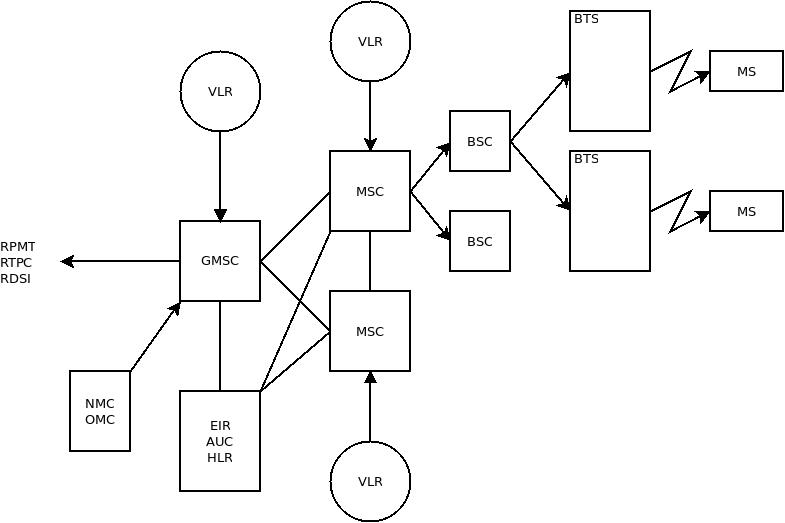
\includegraphics[width=\textwidth]{Imagen/diaGSM.jpg}
\caption{Arquitectura del sistema \acrshort{GSM}}
\label{img:arquiGSM}
\end{figure}
\begin{itemize}
	\item Base Transmission Station (\acrshort{BTS}): Se trata de la antena y los amplificadores de señal, no contiene ningún tipo de "inteligencia", todo se controla desde otros subsistemas.
	\item Mobile Station (\acrshort{MS}): Sistema móvil.
	\item Base Station Controler (\acrshort{BSC}): Controla una o varias \acrshort{BTS} variando potencias transmitidas y canales usados por cada una de ellas.
	\item Mobile Switching Center (\acrshort{MSC}): Controla varias \acrshort{BSC}'s. Están conectadas entre sí en malla.
	\item Gateway Mobile Switching Center (\acrshort{GMSC}): Un \acrshort{MSC} elegido para servir de conexión entre la red móvil y otras redes, como la POTS o Internet. Solo puede haber una por red móvil.
	\item Home Location Register (\acrshort{HLR}): Base de datos de usuarios, contiene la información del \acrshort{MSC} al que se encuentra conectado, datos de tarificación, etc.
	\item Visitor Location Register (\acrshort{VLR}): Cada \acrshort{MSC} tiene uno conectado directamente y se encarga de mantener los datos de usuario de los usuarios conectados a dicho \acrshort{MSC}. Este sistema descarga tráfico del \acrshort{HLR}. Cada vez que un nuevo ususario se registra en el \acrshort{MSC} ha de solicitar su información al \acrshort{HLR}.
	\item Operational Management Center (\acrshort{OMC}): Centro de gestión de características de las \acrshort{BTS}  del sistema.
	\item Network Management Center (\acrshort{NMC}): Centro de gestión de ususarios.
	\item Equipment Identifier Register (\acrshort{EIR}): Base de datos de equipos invalidados, lista negra de moviles robados, basicamente.
	\item Authentication Center: Base de datos con las claves de autenticación de los usuarios del sistema.
	\item Interfaz U: interfaz de conexión radio entre las \acrshort{BTS} y las \acrshort{MS}.
	\item Interfaz de linea o interfaz A: interfaz de conexión entre las \acrshort{MSC} y las \acrshort{BSC}.
	\item Interfaz A-bis: interfaz de conxión entre las \acrshort{BSC} y las \acrshort{BTS}. Esta interfaz surje junto a la idea de conectar varias \acrshort{BTS} a una sola \acrshort{BSC}, en las especifiaciones iniciales esto no era necesario.
\end{itemize}
% subsubsection arquiGSM (end)
\subsubsection{Servicios del sistema \acrshort{GSM}}
\label{ssub:serviciosGSM}
Hay dos servicios básicos. Portadores y teleservicios. Los servicios portadores ofrecen una capacidad de transporte en régimen síncrono/asíncrono en modocircuito o paquete con velocidades hasta 9600bps.Los teleservicios, o servicios ofrecidos por el \acrshort{ISP}, son la telefonía digital a dos velocidades: total a 13kbps o mitad a 6,5kbps, los mensajes cortos y los facsímil, FAX del grupo 3. Algunos ejemplos de servicios suplementarios son, la identificación de llamante, redireccionamiento de llamadas, llamada en espera, buzón de voz, conferencias pluripartitas y la tarificación.
% subsubsection serviciosGSM (end)
\subsubsection{Tramas del sistema \acrshort{GSM}}
\label{ssub:tramaGSM}
Cada trama básica del sistema \acrshort{GSM} está constituida por 8 intervalos de 0,577ms durando la trama 4,615ms en total. Los enlaces descendentes y ascendentes para cada canal están decalados 3 timeslots pudiendo así usarse la misma antena para ambos enlaces. Cada ráfaga está compuesta por 148 bits. estos bits se organizan, como se puede ver en la imagen, de la siguiente forma.
\begin{itemize}
	\item 6 bits de cabecera (Tail Bits).
	\item 116 bits de datos, de los cuales 2 son flags que indican si se trata de un mensaje TCH o \acrshort{FACCH}.
	\item 26 bits de entrenamiento para la estimación del canal y del equalizador.
	\item Un tiempo de guarda equivalente a 8,25 bits. Para la sincronización entre los usuarios.
\end{itemize} 
\begin{figure}[H]
\centering
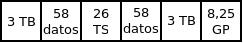
\includegraphics[width=0.6\textwidth]{Imagen/tramaGSM.jpg}
\caption{Estructura de una trama normal de datos de \acrshort{GSM}}
\label{img:tramaGSM}
\end{figure}
Con esta estructura se puede ver que la velocidad de transmisión del enlace radio del sistema \acrshort{GSM} es: $\sfrac{156,25bits}{0,577ms}=270,833kbps$\\
Para reducir la cantidad de señalización necesaria, las tramas se agrupan en multitramas, supertramas e incluso hipertramas. Las supertramas de 26 tramas se usan para los canales de tráfico, las de 51 tramas, en cambio, se usan para canales de señalización y control.
% subsubsection tramaGSM (end)
\subsubsection{Canales del sistema \acrshort{GSM}}
\label{ssub:canalesGSM}
Los canales en \acrshort{GSM} se dividen en canales de tráfico y canales de señalización. Los canales de tráfico siempre vienen definidos por el par de portadoras y timeslots asignados para la comunicación. Se han especificado 7 posibles canales de tráfico:
\begin{itemize}
	\item Voz a velocidad total (TCH/F)
	\item Voz a velocidad mitad (TCH/H)
	\item Datos a velocidad de 2,4, 4,8 y 9,6 kbps
	\item Datos a velocidad mitad de 2,4 y 4,8 kbps
\end{itemize}
Estos canales tienen asociados dos canales de señalización, el \acrshort{SACCH} y el \acrshort{FACCH}. El Slow Associated Control Channel (\acrshort{SACCH}) es el canal que transmite la señalización necesaria para mantener la llamada, como, control de potencia, calidad del canal, tarificación, etc. El Fast Associated Control Channel (\acrshort{FACCH}) es el canal que transmite los mensajes urgentes relacionados con la llamada, como un traspaso de celda. El \acrshort{FACCH} utiliza espacio del canal de información debido al carácter urgente de la información que se transmite en él. A parte hay otros canales de señalización descritos a continuación:
\begin{itemize}
	\item Canales de difusión, canales descendentes que transmiten a todos los terminales móviles informaciones varias.
	\begin{itemize}
		\item Broadcast Control CHannel (\acrshort{BCCH}), transmite información general de la red y la celda para la orientación.
		\item Frecuency Correction CHannel (\acrshort{FCCH}), envía información precisa sobre las portadoras utilizadas por la \acrshort{MS}.
		\item Synchronization CHannel (\acrshort{SCH}), difunde información sobre sincronización de trama e identificación de la \acrshort{BTS}.
	\end{itemize}
	\item Canales comunes (\acrshort{CCH}), se utilizan para regular el acceso al sistema de los terminales. Los hay ascendentes y descendentes.
	\begin{itemize}
		\item Random Acces CHannel (\acrshort{RACH}), canal ascendente usado para la solicitud de recursos al sistema por parte de las \acrshort{MS}. Utiliza el protocolo ALOHA ranurado para controlar el acceso múltiple de las \acrshort{MS} al canal.
		\item Paging CHannel (\acrshort{PCH}), canal descendente por dodne se notifica a las \acrshort{MS}  de una llamada destinada a la misma.
		\item Access Grant CHannel (\acrshort{AGCH}), canal descendente usado para la asignación de canales previamente solicitados por el \acrshort{RACH}.
	\end{itemize}
	\item Los canales dedicados son canales bidireccionales que se asignan a las \acrshort{MS} en exclusiva durante los momentos previos a la llamada.
	\begin{itemize}
		\item Stand-alone Dedicated Control CHannel (SDCCH), se divide en 8 canales vinculados a diferentes \acrshort{MS} para el intercambio de información de señalización.
		\item Slow Associated Control CHannel (\acrshort{SACCH}), es el canal de señalización lenta asociada a la información transmitida por el SDCCH. está dividido en 8 cnanales vinculados a los 8 del SDCCH.
	\end{itemize}
\end{itemize}
% subsubsection canalesGSM (end)
% subsection GSM (end)